\documentclass[a4paper,12pt]{article}
\usepackage{enumerate,amsmath,amssymb,color,graphicx,geometry,hyperref}
\linespread{1.6}
\geometry{margin=2.5cm}
\title{Linear Algebra}
\author{Kathy}
\date{\today}

\begin{document}
\maketitle

\section{Geomatric explaination of matrix}

\subsection{Two geometric ways understanding matrix}

For linear equations:
\begin{equation}
  \label{eq:3}
  \begin{cases}
    2x - y = 0 \\
    -x + 2y = 3
  \end{cases}
\end{equation}

We can write them in matrix multiplication form:
\begin{equation}
  \label{eq:2}
  \begin{bmatrix}
    2 & -1\\
    -1 & 2
  \end{bmatrix}
  \begin{bmatrix}
    x \\ y
  \end{bmatrix}
  = \begin{bmatrix}
    0 \\ 3
  \end{bmatrix}
\end{equation}
where  $\boldsymbol{A}$ is the coefficient matrix, $\boldsymbol{x}$ is the
unknown variable vector, $\boldsymbol{b}$ is the result vector, written as $\boldsymbol{Ax = b}$.

Such kind of form can be understood from two geometric ways:

\begin{enumerate}[(1)]
  \item Row picture form:
    It plots every row function. In two dimentional example they are two linear
equations, each with two unknown variables, i.e. two lines.

  \item Column picture form:
    The plot is presented in column vector way. The purpose is to find a linear
combination that gives the column $\boldsymbol{b}$. Applying all possible
combinations of \textit{x} and \textit{y} produces the two dimentional plane.
But in this case there is only a unique set combination produces $\boldsymbol{b}$.
\end{enumerate}

\begin{figure}[!hbtp]
  \centering
  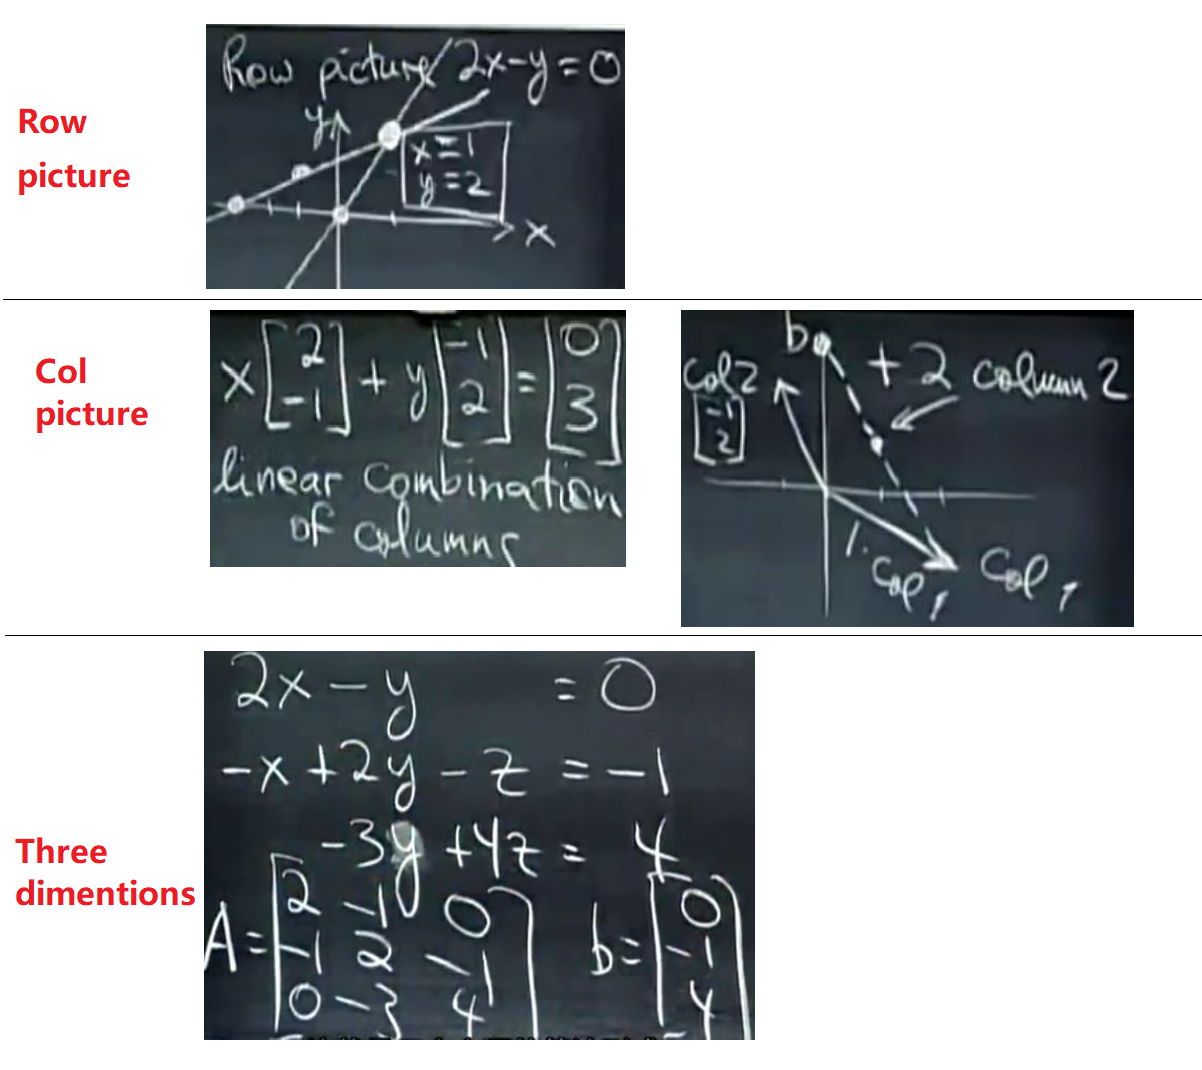
\includegraphics[width=0.75\linewidth]{figures/1.png}
  \caption{Higher Dimensional Examples}
  \label{fig:hd-examples}
\end{figure}

Figure \ref{fig:hd-examples} interpretation applies to higher dimentional examples.

\subsection{The roots of equation sets}

Taking the above three dimentional equation sets as example: when
$\boldsymbol{b}$ is unknown (and the $\boldsymbol{Ax}$ remain unchanged),
whether there is solution for every $\boldsymbol{b}$?

From the column picture explaination, this question is an equavlent of: whether
the linear combinations of columns in $\boldsymbol{A}$ fill up a three
dimentional space?

Answer:
The above case is non-singular matrix, so YES.
For general case, the equation sets {\color{red} only has solution when $\boldsymbol{b}$ is
in the column space spaned by $\boldsymbol{A}$ }.

There are many benefits to consider matrix multiplication in {\color{red} column
picture} way.

\subsection{Appendix}

\end{document}
